% This is a LaTeX template for poster using University of Helsinki style
% This version uses pdflatex; if you have XeTeX available, 
% consider using poster_xetex.tex for fancy font settings
%
% The official Graphical Instructions available from hy.logodomain.com (from university network only) defines colours, fonts etc. This Template does not perfectly match the official poster template of the university
%
% Jukka Suomela's collection of LaTeX tricks has been invaluable in building this template: http://cs.helsinki.fi/u/josuomel/latex/ 
%
% Original template by Janne Korhonen
% This file by Juha Karkkainen

% Encoding of this file is iso-8859-1 latin 1

\documentclass[a4paper]{article} % This actually makes poster of size A4, scale up when printing. Used text font size is a bit small for A1 poster, preferably use \small in that case 

% Misc. packages
\usepackage[T1]{fontenc}
\usepackage{url}
\usepackage{amsfonts}
\usepackage[absolute]{textpos}
\usepackage{amssymb}
\usepackage{amsmath} 
\usepackage{amsthm}

% Graphics stuff
\usepackage[usenames,dvipsnames]{color}
\usepackage{graphicx}


% My favourite macros
\newcommand{\N}{\mathbb{N}} %natural numbers
\newcommand{\Z}{\mathbb{Z}} %integers
\newcommand{\Q}{\mathbb{Q}} %rationals
\newcommand{\R}{\mathbb{R}} %reals

\newcommand{\G}{\mathcal{G}} % fancy G
\newcommand{\A}{\mathcal{A}} % fancy A
\newcommand{\bO}{\mathcal{O}} % fancy O

\newcommand{\eos}{\#}
\newcommand{\rank}{\textsc{rank}}


% enumitem for controlling enumerate and itemize environments; usefull for saving space
\usepackage{enumitem}


% Fonts
%
% Palantino - Helvetica - Courier.
% I haven't really spent time to figure out how to best match the official university style with latex font packages, as I use XeTex myself...
\usepackage{mathpazo}
\linespread{1.10}
\usepackage[scaled]{helvet}
\usepackage{courier}

% Colours
\definecolor{sciorange}{RGB}{252,163,17}
\definecolor{unigray}{RGB}{140,140,140}
\definecolor{first}{RGB}{180,30,10}
\definecolor{second}{RGB}{10,120,130}
\definecolor{new}{RGB}{190,50,10}
\definecolor{wavelet}{RGB}{70,140,220}
%\definecolor{improved}{RGB}{80,200,80}
\definecolor{improved}{RGB}{10,100,160}
\definecolor{prior}{RGB}{140,140,140}

% Textpos to manually position blocks of text on the page
\usepackage[absolute]{textpos}

% We define 1 mm grid for positioning the text blocks on the page
% The idea is to leave 10 mm marginals to all sides; the three text columns are 60 mm wide with 5 mm space between columns.
\setlength{\TPHorizModule}{1mm}
\setlength{\TPVertModule}{1mm}

% The origin is set to right below the main title; this means that main title blocks have negative y-coordinate. There is actually no good reason for this, I just happened to do this that way.
\textblockorigin{10mm}{48.5mm}


% parindent is set to zero, because it looks better in posters
% you could also add some space between paragraphs here, but I use manual vertical spaces in this sample
\setlength{\parindent}{0pt}

%Nice table cell formatting for multirow cells:
\newcommand{\specialcell}[2][c]{%
  \begin{tabular}[#1]{@{}c@{}}#2\end{tabular}}
\usepackage{multicol}
 


% Finally, the content
\begin{document}
\pagestyle{empty} % To get rid of page numbers and so

% ------------------------------------------------------------------------------------------------------------------------------
% Main title, University logo etc.
 
% If you need more space for the title or want the logo to be bigger, you need to adjust various parameters, as I did not bother to automate this yet
% Mainly, move the textblockorigin above down and adjust all the boxes here to be higher up.

% First, the University logo. The included flame.pdf is a copy of the official logo in vector format, so it is good for all sizes.
% Box starts 10 mm from the top
\begin{textblock}{95}(0,-38.5)

\includegraphics[width=22mm]{flame}
\end{textblock} 

% University - Faculty - Department
% Box starts 10 mm from the top
\begin{textblock}{95}(95,-38.5)
{\fontsize{8}{7}\selectfont\sffamily\color{unigray}
\hfill HELSINGIN YLIOPISTO

\hfill HELSINGFORS UNIVERSITET

\hfill UNIVERSITY OF HELSINKI

\color{sciorange}\hfill MATEMAATTIS-LUONNONTIETEELLINEN TIEDEKUNTA

\hfill MATEMATISK-NATURVETENSKAPLIGA FAKULTETEN

\hfill FACULTY OF SCIENCE % For some reason, the last line here gets messed up without extra spaces...


}
\end{textblock}


% Main title
% If you need two lines for the title, you need to adjust the position of this block and textblockorigin
% Remember, two first words use faculty colour. If your title is long, you can use small letters.
\begin{textblock}{190}(0,-13.5)
{\sffamily\LARGE{\color{sciorange}String Sorting in Python -- }{\color{unigray}
 Comparison of Several Algorithms}}\\
\small\hfill Onni Koskinen, Arturs Polis, and Lari Rasku\\ % If you have multiple authors, their names can be on the same line. Adjust font size as necessary
\rule[2mm]{190mm}{0.3pt} % This is the line under the title, adjust the last parameter if it seems to be in the wrong place
\end{textblock}

% ------------------------- TEST DATA SET  ----------------------------------
\begin{textblock}{100}(0,5)
    \sffamily\normalsize{\color{sciorange}TESTING DATA}\small\\
 \footnotesize 
\begin{table}
    \begin{tabular}{| l | l | l | l | l | l |}
    \hline
    \specialcell{Dataset} & \specialcell{Number \\ of strings} &\specialcell{Sum of\\ lengths}& \specialcell{Max \\ string length} & \specialcell{alphabet \\ size}&  \specialcell{Sum of \\ LCP array}  \\ 
    \hline
    dna.100MB&  618&    104856983&  3732300&    15& 4501\\
    dna.200MB&  1114&   209714087&  3732300&    15& 8948\\
    proteins.100MB& 359505& 104498096&  36805&  24& 18853436\\
    proteins.200MB& 709116& 209006085&  36805&  24& 50076184\\
    urls.100MB& 3284368&    101569109&  372&    114&    94113004\\
    urls.200MB& 6576059&    203139142&  560&    114&    191545831\\
    words.100MB&    18502734&   85200064&   112&    211&    83643408\\
    words.200MB&    37003241&   170395992&  112&    220&    168115390\\
    \hline
    \end{tabular}
\caption{Data set used for comparing the algorithms}
\label{dataset}
\end{table}

\end{textblock} 

% ---------------------------- RESULTS DATA----------------------------------
\begin{textblock}{120}(0,180)
    \sffamily\normalsize{\color{sciorange}TEST RESULTS}\small
\footnotesize 
\begin{table}
    \begin{center}
        \begin{tabular}{| l | l | l | l | l | l | l | l | l | l | l | l | l |}
        \hline
Algorithm: & \multicolumn{2}{|c|}{sorted (python builtin)} & \multicolumn{2}{|c|}{Radixsort - MSD} & \multicolumn{2}{|c|}{Multikey QuickSort} &\multicolumn{2}{|c|}{TernaryQuickSort} & \multicolumn{2}{|c|}{Burstsort}  &  \multicolumn{2}{|c|}{In-place QuickSort}\\ \hline 
Time:   &  real&   user&   real&   user&   real&   user&   real&   user&   real&   user&   real&   user\\ \hline
dna.100MB&  0.297&  0.2&0.346&  0.284&  0.34&   0.276&  0.332&  0.276&  4.604&  1.284&  1.527&  1.28\\
dna.200MB&  0.498&  0.372&  0.639&  0.532&  0.633&  0.52&   0.637&  0.52&   2.808&  2.44&   2.941&  2.484\\
proteins.100MB& 0.841&  0.768&  7.126&  7.024&  7.293&  7.2&1.996&  1.908&  9.189&  8.705&  4.505&  4.252\\
proteins.200MB& 1.651&  1.532&  21.095& 20.921& 23.467& 23.301& 3.445&  3.272&  25.551& 24.67&  11.271& 10.793\\
urls.100MB& 5.209&  5.072&  11.132& 10.893& 25.299& 25.062& 8.815&  8.585&  8.508&  8.185&  5.617&  5.348\\
urls.200MB& 10.889& 10.601& 22.208& 21.641& 65.46&  64.836& 17.437& 16.921& 16.843& 16.245& 12.257& 11.697\\
words.100MB&22.159& 21.449& 21.126& 20.357& 127.363&125.384&35.637& 34.182& 9.486&  9.193&  13.865& 13.313\\
words.200MB&46.719& 45.311& 43.636& 42.147& 371.045&367.687&77.147& 71.788& 17.897& 17.361& 28.151& 27.09\\
        \hline
        \end{tabular}
    \end{center}
    \caption{Algorithm running times}
    \label{dataset}
\end{table}


\end{textblock}

% ----------------------- ALGORITHMS ----------------------------

%\begin{textblock}{125}(0,97)
\sffamily\normalsize{\color{sciorange}ALGORITHMS}\small\\
\rule[3mm]{125mm}{0.1pt}
\end{textblock} 

%leaving the column location definitions outside of the actual content
\begin{textblock}{60}(0,103)
    {\sffamily\normalsize{\color{sciorange} MSD RADIX SORT}}\vspace{1mm}\\
\footnotesize 
MSD radix sort first partitions the strings into different buckets based on
first symbol is, then recursively partitions *those* buckets based on what
the second symbol is, and so on.  When only single-element buckets or buckets
containing only strings shorter than the recursion depth are left, the results
are concatenated and output.\\

{\em Highlight and underline these to illustrate the partitioning.}
\begin{quote}
    {\color{green}a}ctor\\
    {\color{sciorange}al}locate\\
    {\color{sciorange}al}pha\\
    {\color{red}b}eta\\
    {\color{red}b}yproduct\\
\end{quote}
MSD radix sort never needs to process a symbol twice, technically giving it
$O(L(R) + n)$ complexity assuming a finite alphabet.  However, the complexity
is dominated by the bucket container data structure: if $\sigma$ is the size of the
alphabet and if the buckets are stored in a binary search tree, each addition
takes $O(\log \sigma)$ time.  If they are stored in an array or a hash table, merging
takes $\Theta(\sigma)$ time.
    {\sffamily\normalsize{\color{sciorange} QUICKSORT ALGORITHMS}}\vspace{1mm}\\
\footnotesize 
Quicksort text  
Quicksort text 
Quicksort text  
Quicksort text 
Quicksort text  
Quicksort text 
Quicksort text  
Quicksort text 
Quicksort text  
Quicksort text 
Quicksort text  
Quicksort text 
Quicksort text  
Quicksort text 
Quicksort text  
Quicksort text 
\end{textblock}

\begin{textblock}{60}(65,103)
    {\sffamily\normalsize{\color{sciorange} BURST SORT}}\vspace{1mm}\\
\footnotesize 
Burst sort text    
Burst sort text    
Burst sort text    

Burst sort text    
Burst sort text    
Burst sort text    
Burst sort text    
Burst sort text    

Burst sort text    
Burst sort text    

Burst sort text    
Burst sort text    

Burst sort text   

\end{textblock}
	
%---------------------- RIGHT COLUMN ------------------------------
% Third column
\begin{textblock}{60}(130,5)
     \begin{textblock}{60}(130,20)
  {\sffamily\normalsize{\color{sciorange}
      EXPERIMENTAL RESULTS}}\vspace{1mm}\\
  \footnotesize 
  The graphs below show the time and space requirements of several
  algorithms on two texts.  The algorithms are divided
  into three groups:
  \begin{description}
  \item[\color{new}New] algorithms based on reference point ranks, repetition
    shortcuts and wavelet trees
  \item[\color{improved}Improved] implementations of wavelet trees and
    algorithms from~\cite{ll2005}
  \item[\color{prior}Prior] algorithms from~\cite{s2001,ll2005}
  \end{description}
  \vspace{2mm}

  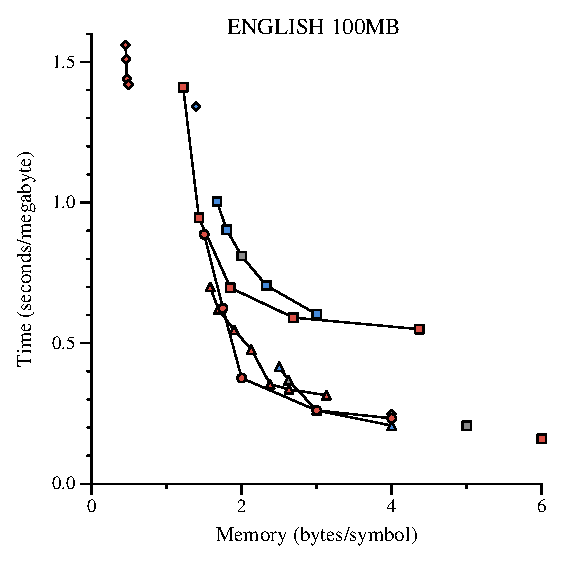
\includegraphics[width=60mm]{eng100Mb-new}
  \vspace{2mm}

  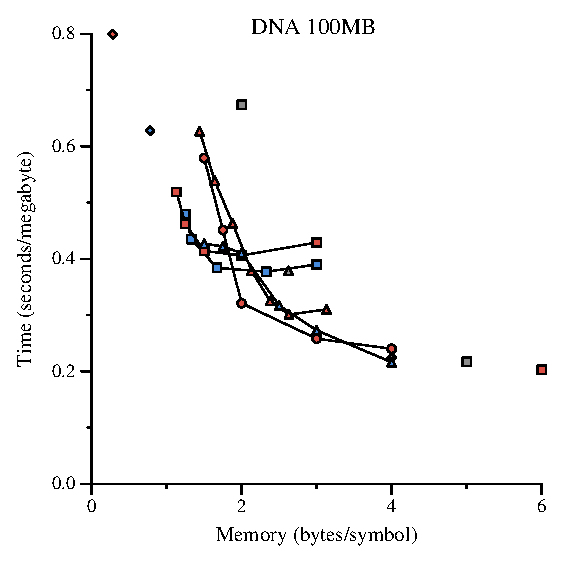
\includegraphics[width=60mm]{dna100Mb-new}
\end{textblock}

\end{textblock}

% \begin{textblock}{60}(130,20)
  {\sffamily\normalsize{\color{sciorange}
      EXPERIMENTAL RESULTS}}\vspace{1mm}\\
  \footnotesize 
  The graphs below show the time and space requirements of several
  algorithms on two texts.  The algorithms are divided
  into three groups:
  \begin{description}
  \item[\color{new}New] algorithms based on reference point ranks, repetition
    shortcuts and wavelet trees
  \item[\color{improved}Improved] implementations of wavelet trees and
    algorithms from~\cite{ll2005}
  \item[\color{prior}Prior] algorithms from~\cite{s2001,ll2005}
  \end{description}
  \vspace{2mm}

  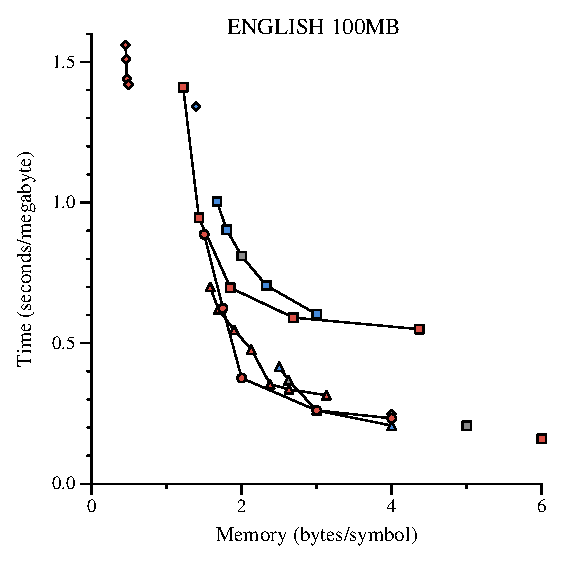
\includegraphics[width=60mm]{eng100Mb-new}
  \vspace{2mm}

  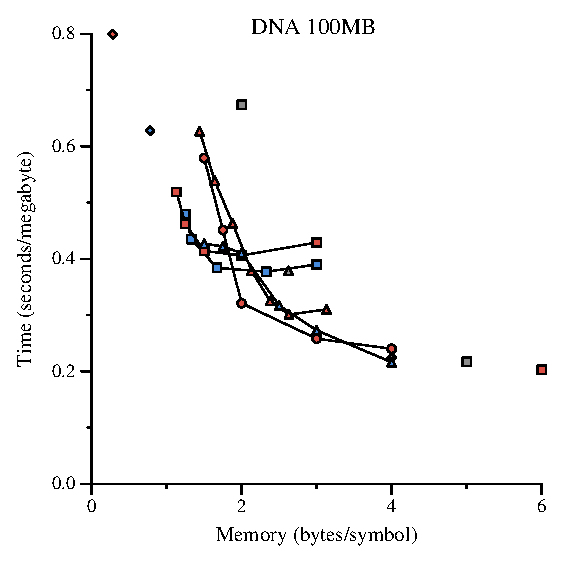
\includegraphics[width=60mm]{dna100Mb-new}
\end{textblock}


%\begin{textblock}{60}(130,165)
%  {\sffamily\normalsize{\color{sciorange}CONCLUDING REMARKS}}\vspace{1mm}\\
%  \footnotesize 
%\end{textblock}

%\begin{textblock}{180}(0, 205)
%  \def\refname{\normalfont\sffamily\normalsize{\color{sciorange}REFERENCES}}
%  \scriptsize\sffamily
%  \bibliographystyle{abbrv}
%  \bibliography{poster}
%\end{textblock}
% Unfortunately, this template has no references. The official instructions seem to indicate that sans-serif font is used for the reference list.

\end{document}
